% \documentclass{myreport}% 选项 forprint: 交付打印时添加, 避免彩色链接字迹打印偏淡. 即使用下一行:
% \documentclass[forprint]{myreport}
\documentclass{myreport}

\usepackage{tcolorbox}
\usepackage{listings}
% \usepackage{float}
\usepackage[section]{placeins}


\lstdefinestyle{lfonts}{
    basicstyle = \footnotesize\ttfamily,
    stringstyle = \color{purple},
    keywordstyle = \color{blue!60!black}\bfseries,
    commentstyle = \color{olive}\scshape,
}
\lstdefinestyle{lnumbers}{
    numbers = left,
    numberstyle = \tiny,
    numbersep = 1em,
    firstnumber = 1,
    stepnumber = 1,
}
\lstdefinestyle{llayout}{
    breaklines = true,
    tabsize = 2,
    columns = flexible,
}
\lstdefinestyle{lgeometry}{
    xleftmargin = 20pt,
    xrightmargin = 0pt,
    frame = tb,
    framesep = \fboxsep,
    framexleftmargin = 20pt,
}
\lstdefinestyle{lgeneral}{
    style = lfonts,
    style = lnumbers,
    style = llayout,
    style = lgeometry,
}
\lstdefinestyle{c}{
	language = {c},
	style = lgeneral,
}
\setcounter{tocdepth}{3}

\begin{document}
%%%%%%%%%%%%%%%%%%%%%%%%%%%%%%%%%%%%%%%%%%%%%%%%%%%%%%%%%%%%%%%%%%%%%%%%%%%%%
% 封面
%%%%%%%%%%%%%%%%%%%%%%%%%%%%%%%%%%%%%%%%%%%%%%%%%%%%%%%%%%%%%%%%%%%%%%%%%%%%%
\title{计算机网络实验四:\\ 虚拟局域网配置}% TODO:标题
\Cschoolname{数据科学与计算机学院}          % 学院名
\Cmajor{计算机科学与技术}                  % 专业中文名
\StudentNumber{16337237,16337269,16337271} % 填写自己的学号
\author{王永锋,颜彬,杨陈泽}                            % 作者名字
\Csupervisor{陈立文}    %指导教师中文名、职称
\date{二〇一八年五月十五日} % TODO:               % 日期, 要注意和英文日期一致!!
\pdfbookmark[0]{封面}{title}         % 封面页加到 pdf 书签
\maketitle
\frontmatter
%%%%%%%%%%%%%%%%%%%%%%%%%%%%%%%%%%%%%%%%%%%%%%%%%%%%%%%%%%%%%%%%%%%%%%%%%%%%%
% 目录
%%%%%%%%%%%%%%%%%%%%%%%%%%%%%%%%%%%%%%%%%%%%%%%%%%%%%%%%%%%%%%%%%%%%%%%%%%%%%
% 把目录加入到书签
\pagenumbering{Roman}              % 正文之前的页码用大写罗马字母编号.
\pdfbookmark[0]{目录}{toc}
\tableofcontents
%% 以下是正文
\mainmatter 
%%%%%%%%%%%%%%%%%%%%%%%%%%%%%%%%%%%%%%%%%%%%%%%%%%%%%%%%%%%%%%%%%%%%%%%%%%%%
% 正文
%%%%%%%%%%%%%%%%%%%%%%%%%%%%%%%%%%%%%%%%%%%%%%%%%%%%%%%%%%%%%%%%%%%%%%%%%%%%
\chapter{小组成员及分工}

\section{小组成员}

\begin{table}[htp]
  \caption{小组成员信息}
  \centering
  \rowcolors{1}{White}{Lavender}
  \begin{tabular}{cc}
  \toprule
  组员姓名 & 学号 \\
  \midrule
  王永锋(组长) & 16337237 \\
  颜彬 & 16337269 \\
  杨陈泽 & 16337271 \\
  \bottomrule
  \hiderowcolors
\end{tabular}
\label{tab:group}
\end{table}

\section{小组分工表及自评}
\begin{table}[htp]
  \caption{小组分工表}
  \centering
  \rowcolors{1}{White}{Lavender}
  \begin{tabular}{lcp{11cm}}
    \toprule
    小组成员姓名 & 自评 & 分工 \\
    \midrule
    王永锋 & 100 & TODO: 及实验报告排版 \\
    颜彬 & 100 & TODO:\\
    杨陈泽 & 100 & TODO:分工 \\
  \bottomrule
  \hiderowcolors
  \end{tabular}
  \label{tab:group-devide}
\end{table}
%%%%%%%%%%%%%%%%%%%%%%%%%%%%%%%%%%%%%%%%%%%%%%%%%%%%%%%%%%%%%%%%%%%%%%%%%%%%
% 实验一:跨交换机的VLAN
%%%%%%%%%%%%%%%%%%%%%%%%%%%%%%%%%%%%%%%%%%%%%%%%%%%%%%%%%%%%%%%%%%%%%%%%%%%%
\chapter{实验一:跨交换实现VLAN}

\section{实验拓扑}

TODO:画一个拓扑图,这个图和书本的图一样。

PC1,我 
PC2,颜彬
PC3,陈泽

\section{实验步骤}

\subsection{步骤1}

将我们的三台电脑按照拓扑图配置好IP地址,用网线将各电脑与交换机对应的端口相连。

然后检测三台电脑间能否互相ping通,下\autoref{fig:e1-s1-ping}展示了PC1 \texttt{ping} PC2 与PC3的结果,都能够ping通,表明网络线路没有问题。

%\usepackage{changepage}
%\usepackage{rotating}
%\begin{sidewaystable}[htp]
\begin{figure}[htp]
    %\begin{adjustwidth}{-1.5cm}{-1cm}
    \centering
    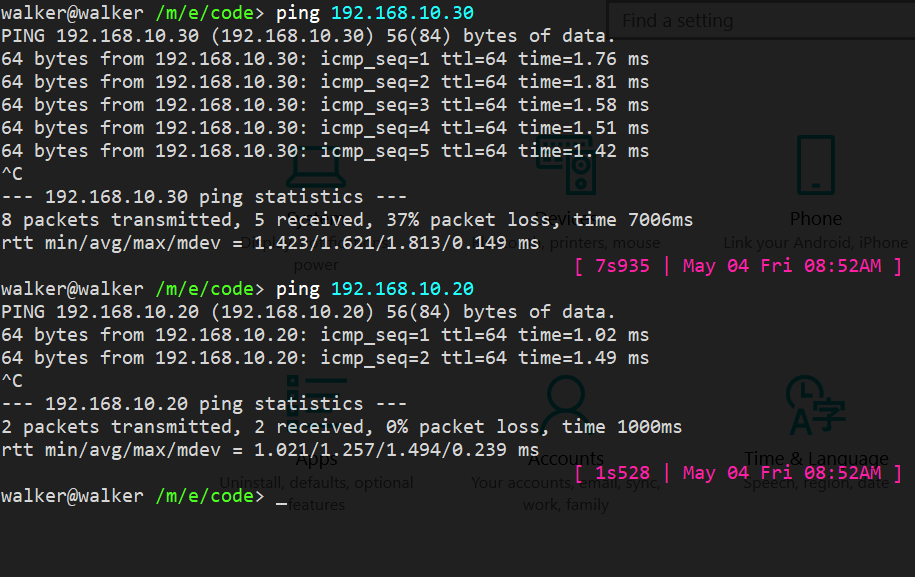
\includegraphics[width=13cm]{"./figure/2018-05-04-08-53-24.png"}
    \caption{PC1 ping PC2 PC3}
    \label{fig:e1-s1-ping}
    %\end{adjustwidth}
\end{figure}

\subsection{步骤2:路由器1设置vlan10}

该步骤需要路由器1将PC1对应的端口(gig 0/5)设置为vlan 10。

相关设置的步骤可见\autoref{fig:e1-s2-10}。

%\usepackage{changepage}
%\usepackage{rotating}
%\begin{sidewaystable}[htp]
\begin{figure}[htp]
    %\begin{adjustwidth}{-1.5cm}{-1cm}
    \centering
    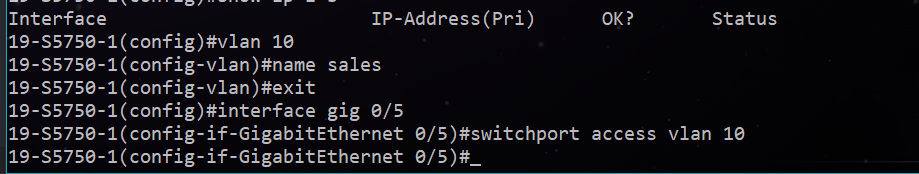
\includegraphics[width=13cm]{"./figure/2018-05-04-09-10-21.png"}
    \caption{路由器1设置PC1端口为vlan 10}
    \label{fig:e1-s2-10}
    %\end{adjustwidth}
\end{figure}

完成设置后,由于PC1在VLAN 10中,而PC2,PC3在默认的VLAN1中,如果设置成功的话是PC2是无法ping通PC1的,下面进行验证。

\begin{enumerate}
    \item 使用指令\texttt{show vlan id 10}查看vlan10对应的端口,可见\autoref{fig:e1-s2-check-1}
    %\usepackage{changepage}
    %\usepackage{rotating}
    %\begin{sidewaystable}[htp]
    \begin{figure}[htp]
        %\begin{adjustwidth}{-1.5cm}{-1cm}
        \centering
        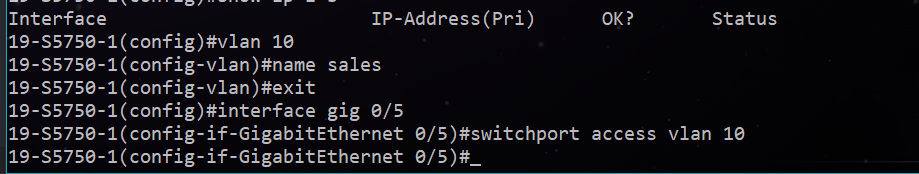
\includegraphics[width=13cm]{"./figure/2018-05-04-09-10-21.png"}
        \caption{查看VLAN 10对应的端口}
        \label{fig:e1-s2-check-1}
        %\end{adjustwidth}
    \end{figure}
    \item PC2 无法ping通PC1,可见\autoref{fig:e1-s2-check-ping}.
    %\usepackage{changepage}
    %\usepackage{rotating}
    %\begin{sidewaystable}[htp]
    \begin{figure}[htp]
        %\begin{adjustwidth}{-1.5cm}{-1cm}
        \centering
        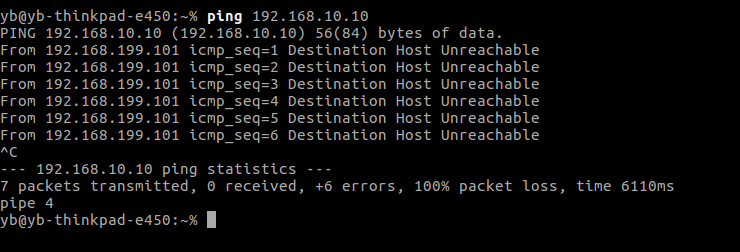
\includegraphics[width=13cm]{"./figure/id001.png"}
        \caption{PC2 无法 ping 通 PC1}
        \label{fig:e1-s2-check-ping}
        %\end{adjustwidth}
    \end{figure}
\end{enumerate}


\section{步骤3:设置路由器1设置 VLAN 20}

该步骤要求将PC2对应的交换机的端口设置为VLAN 20。这时候,原本能够相互ping通的PC2与PC3也开始不能相互ping通。

相关设置的步骤可见\autoref{fig:e1-s3-vlan-20}.

%\usepackage{changepage}
%\usepackage{rotating}
%\begin{sidewaystable}[htp]
\begin{figure}[!htp]
    %\begin{adjustwidth}{-1.5cm}{-1cm}
    \centering
    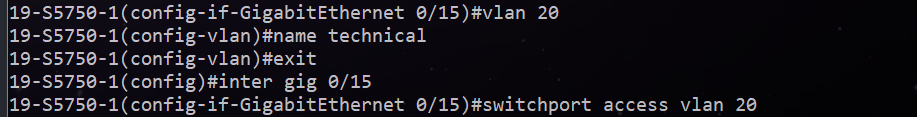
\includegraphics[width=13cm]{"./figure/2018-05-04-09-18-39.png"}
    \caption{设置VLAN 20}
    \label{fig:e1-s3-vlan-20}
    %\end{adjustwidth}
\end{figure}

设置后,我们进行验证,查看路由器的配置与检查PC2与PC3是否能够ping通。

\begin{enumerate}
    \item 使用指令\texttt{show vlan id 20}查看vlan20对应的端口,可见\autoref{fig:e1-s3-check-1}
    %\usepackage{changepage}
    %\usepackage{rotating}
    %\begin{sidewaystable}[htp]
    \begin{figure}[!htp]
        %\begin{adjustwidth}{-1.5cm}{-1cm}
        \centering
        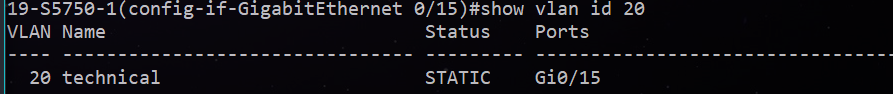
\includegraphics[width=13cm]{"./figure/2018-05-04-09-18-49.png"}
        \caption{查看VLAN 20对应的端口}
        \label{fig:e1-s3-check-1}
        %\end{adjustwidth}
    \end{figure}
    \item PC2 无法ping通PC3,可见\autoref{fig:e1-s3-check-ping}.
    %\usepackage{changepage}
    %\usepackage{rotating}
    %\begin{sidewaystable}[htp]
    \begin{figure}[!htp]
        %\begin{adjustwidth}{-1.5cm}{-1cm}
        \centering
        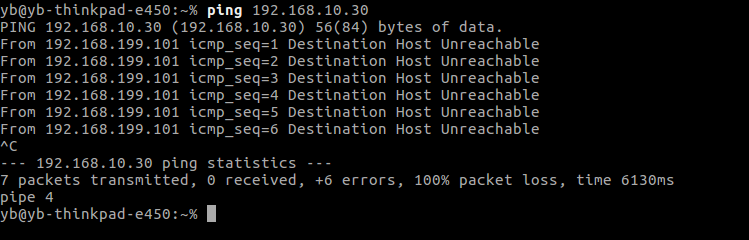
\includegraphics[width=13cm]{"./figure/id002.png"}
        \caption{PC2 无法 ping 通 PC3}
        \label{fig:e1-s3-check-ping}
        %\end{adjustwidth}
    \end{figure}
\end{enumerate}

\section{步骤4::设置路由器1端口的trunk模式}

该步骤要求设置两路由器相连的端口(0/24)设置为\texttt{trunk}模式。设置步骤可见\autoref{fig:e1-s4-trunk}。

%\usepackage{changepage}
%\usepackage{rotating}
%\begin{sidewaystable}[htp]
\begin{figure}[!htp]
    %\begin{adjustwidth}{-1.5cm}{-1cm}
    \centering
    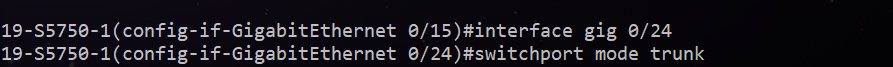
\includegraphics[width=13cm]{"./figure/2018-05-04-09-23-00.png"}
    \caption{将路由器1的0/24端口设置为trunk模式}
    \label{fig:e1-s4-trunk}
    %\end{adjustwidth}
\end{figure}

设置完成后,使用\texttt{show interface gig 0/24 switchport}该指令验证,可见\autoref{fig:e1-s4-check}。

%\usepackage{changepage}
%\usepackage{rotating}
%\begin{sidewaystable}[htp]
\begin{figure}[!htp]
    %\begin{adjustwidth}{-1.5cm}{-1cm}
    \centering
    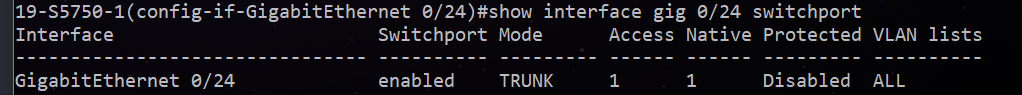
\includegraphics[width=13cm]{"./figure/2018-05-04-09-23-29.png"}
    \caption{验证路由器1的trunk设置}
    \label{fig:e1-s4-check}
    %\end{adjustwidth}
\end{figure}


这个时候由于路由器2上的端口尚未设置,因此仍然不能够ping通。

\section{步骤5:设置路由器2}

由于设置路由器2的指令与设置路由器1的指令类似,这里并不放设置的截图,仅放验证的截图。

由\autoref{fig:e1-s5-vlan20}可知,该次设置成功。

%\usepackage{changepage}
%\usepackage{rotating}
%\begin{sidewaystable}[htp]
\begin{figure}[htp]
    %\begin{adjustwidth}{-1.5cm}{-1cm}
    \centering
    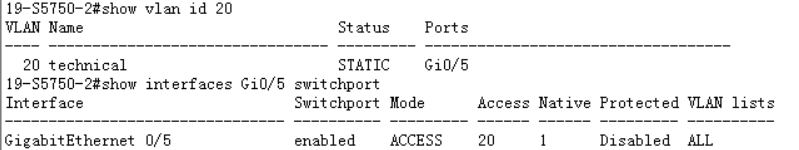
\includegraphics[width=13cm]{"./figure/2018-05-04-10-12-46.png"}
    \caption{验证路由器2的vlan20设置}
    \label{fig:e1-s5-vlan20}
    %\end{adjustwidth}
\end{figure}

此时PC2,PC3之间仍不能够ping通。

\section{步骤6:设置路由器2端口的trunk模式}

路由器2的\texttt{gigabitethernet 0/24}端口与路由器1之间相连,需要设置为\texttt{trunk}模式用以转发链路帧,设置后,验证设置如\autoref{fig:e1-s6-trunk},可知设置成功。

%\usepackage{changepage}
%\usepackage{rotating}
%\begin{sidewaystable}[htp]
\begin{figure}[htp]
    %\begin{adjustwidth}{-1.5cm}{-1cm}
    \centering
    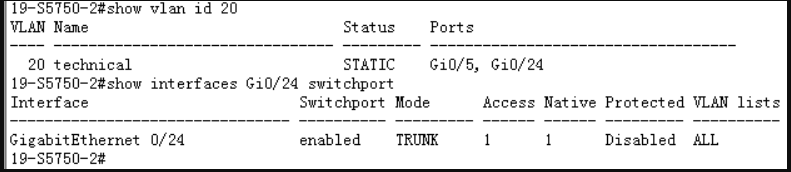
\includegraphics[width=13cm]{"./figure/2018-05-04-10-13-08.png"}
    \caption{验证PC2的trunk模式设置}
    \label{fig:e1-s6-trunk}
    %\end{adjustwidth}
\end{figure}

\section{步骤7:验证}

这一个步骤我们需要验证PC2与PC3之间能相互通信,但PC1与PC3不能相互通信。

因此我们完成了以下几个问题

%\usepackage{tcolorbox}
%\newtcolorbox{mybox}{}
%\renewtcolorbox{mybox}{colback = red!25!white, colframe = red!75!black}
%\begin{mybox}[title = {}]
\begin{tcolorbox}[title = {观察一}]
主机之间能否互相通信?
\end{tcolorbox}
TODO:需要互ping的图
wyf
%\usepackage{tcolorbox}
%\newtcolorbox{mybox}{}
%\renewtcolorbox{mybox}{colback = red!25!white, colframe = red!75!black}
%\begin{mybox}[title = {}]
\begin{tcolorbox}[title = {观察二}]
    能否检测到PC1,PC2,PC3的ICMP包?
\end{tcolorbox}
TODO:分析yb???????

%\usepackage{tcolorbox}
%\newtcolorbox{mybox}{}
%\renewtcolorbox{mybox}{colback = red!25!white, colframe = red!75!black}
%\begin{mybox}[title = {}]
\begin{tcolorbox}[title = {观察三}]
能否捕获到Trunk链路上的VLAN ID?请讨论原因。
\end{tcolorbox}
TODO:分析yb

%\usepackage{tcolorbox}
%\newtcolorbox{mybox}{}
%\renewtcolorbox{mybox}{colback = red!25!white, colframe = red!75!black}
%\begin{mybox}[title = {}]
\begin{tcolorbox}[title = {观察四}]
    
    \begin{itemize}
        \item 查看交换机的地址表。清楚地址表,适当更改、增加网线接口,然后观察,分析地址表的形成与变化过程(配合wireshark分析泛洪现象)。
        \item show mac-address-table命令显示的MAC地址与在命令提示符下通过\texttt{ifconfig /all}命令显示的 \texttt{mac}地址是否相同。
    \end{itemize}
    
\end{tcolorbox}
TODO:颜彬负责

%\usepackage{tcolorbox}
%\newtcolorbox{mybox}{}
%\renewtcolorbox{mybox}{colback = red!25!white, colframe = red!75!black}
%\begin{mybox}[title = {}]
\begin{tcolorbox}[title = {观察五}]
判断实验是否达到预期目标。
\end{tcolorbox}

TODO:吹水?yb

\section{实验思考}

思考题来自于老师的pdf材料.

%\usepackage{tcolorbox}
%\newtcolorbox{mybox}{}
%\renewtcolorbox{mybox}{colback = red!25!white, colframe = red!75!black}
%\begin{mybox}[title = {}]
\begin{tcolorbox}[title = {思考题一}]
说明vlan技术中的trunk模式端口的意义。
\end{tcolorbox}

TODO:yb

\begin{tcolorbox}[title = {思考题二}]
如何查看trunk接口允许哪些VLAN通过?
\end{tcolorbox}
TODO:wyf

\begin{tcolorbox}[title = {思考题三}]
实验开始前请先确定三台PC机处于一个网段里面。为什么做这样的限定?
\end{tcolorbox}
TODO:wyf


\chapter{实验二:通过三层交换机实现VLAN间路由}

\section{实验拓扑}

TODO:书本图片P177

\section{实验步骤}

分析:本实验的预期是将\autoref{TODO:拓扑图}中的三台计算机,划分进不同的VLAN,并让处于不同VLAN的计算机互相隔离.然后启用三层交换机的路由功能,让已经隔离的计算机能互相通信.
(如:隔离后PC1能ping通PC2,PC3).

\subsection{步骤1:连接线路并测试连通性}

\begin{enumerate}
    \item 设置每一台主机的IP地址
    %\usepackage{changepage}
    %\usepackage{rotating}
    %\usepackage{float}
    %\usepackage[section]{placeins}
    %\begin{sidewaystable}[!Htp]
    \begin{figure}[htp]
        %\begin{adjustwidth}{-1.5cm}{-1cm}
        \centering
        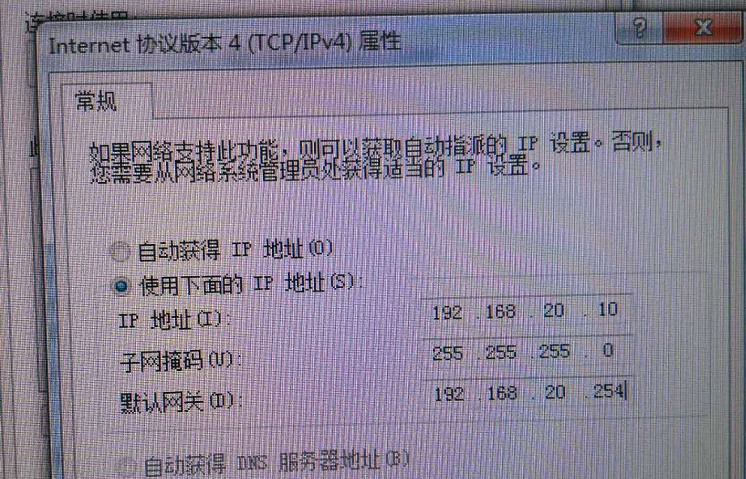
\includegraphics[width=13cm]{"./figure/2018-05-17-22-31-49.png"}
        \caption{PC1设置IP地址的截图}
        \label{fig:e2-s2-set-ip}
        %\end{adjustwidth}
    \end{figure}
    
    \item 测试PC1, PC2, PC3的连通性,发现PC1无法ping通PC2,PC3,其他的PC2和PC3可以相互ping通。
    %\usepackage{tcolorbox}
    %\newtcolorbox{mybox}{}
    %\renewtcolorbox{mybox}{colback = red!25!white, colframe = red!75!black}
    %\begin{mybox}[title = {}]
    %\usepackage{changepage}
    %\usepackage{rotating}
    %\usepackage{float}
    %\usepackage[section]{placeins}
    %\begin{sidewaystable}[!Htp]
    \begin{figure}[htp]
        %\begin{adjustwidth}{-1.5cm}{-1cm}
        \centering
        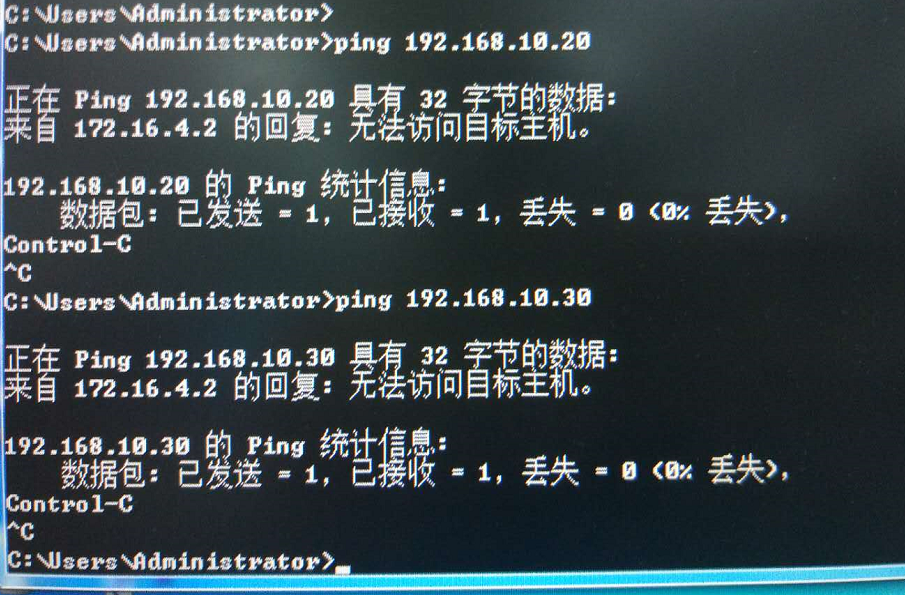
\includegraphics[width=13cm]{"./figure/2018-05-17-22-32-57.png"}
        \caption{PC1无法ping通PC2,PC3}
        \label{fig:e2-s2-not-ping}
        %\end{adjustwidth}
    \end{figure}
    
    \begin{tcolorbox}[title = {思考}]
    PC1的网段不同于PC2,PC3,请讨论原因
    \tcblower
    这里做的是不同vlan间通过路由转发消息的实验。如果PC1与PC2,PC3所在网段相同,那么PC1在发送IP包的时候就会认为在同一个子网中,永远也不会发往默认网关。
    \end{tcolorbox}
    \item 使用\texttt{show ip route}命令查看三层交换机的路由表,并记录
    %\usepackage{changepage}
    %\usepackage{rotating}
    %\usepackage{float}
    %\usepackage[section]{placeins}
    %\begin{sidewaystable}[!Htp]
    \begin{figure}[htp]
        %\begin{adjustwidth}{-1.5cm}{-1cm}
        \centering
        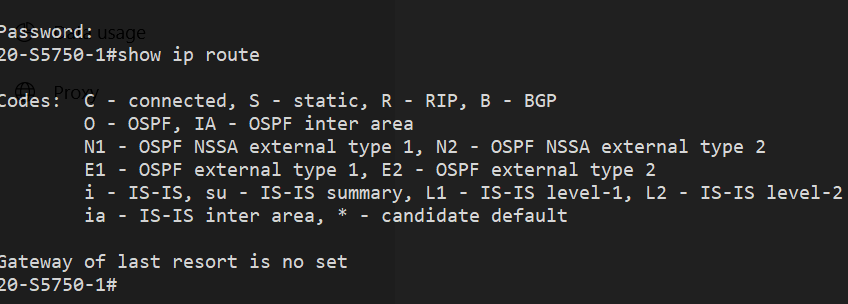
\includegraphics[width=13cm]{"./figure/2018-05-17-17-00-58.png"}
        \caption{查看三层交换机的路由表}
        \label{fig:e2-s1-route}
        %\end{adjustwidth}
    \end{figure}
    

\end{enumerate}

\subsection{步骤2:交换机A创建VLAN10}

该步骤需要在交换机A上创建VLAN10,并将端口0/5(即PC1对应的接口)划分到VLAN10中.

%\usepackage{changepage}
%\usepackage{rotating}
%\usepackage{float}
%\usepackage[section]{placeins}
%\begin{sidewaystable}[!Htp]
\begin{figure}[htp]
    %\begin{adjustwidth}{-1.5cm}{-1cm}
    \centering
    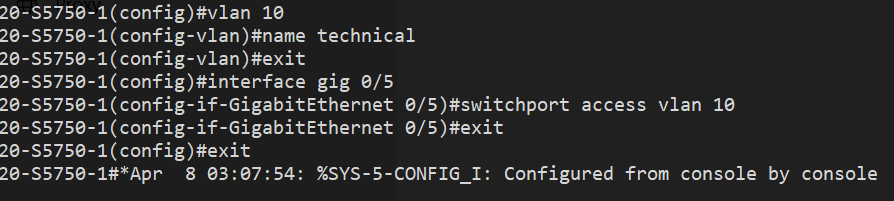
\includegraphics[width=13cm]{"./figure/2018-05-17-17-03-01.png"}
    \caption{交换机A创建VLAN 10}
    \label{fig:e2-s2-vlan10}
    %\end{adjustwidth}
\end{figure}


操作完成后,使用\texttt{show vlan id 10}验证实验操作.

%\usepackage{changepage}
%\usepackage{rotating}
%\usepackage{float}
%\usepackage[section]{placeins}
%\begin{sidewaystable}[!Htp]
\begin{figure}[htp]
    %\begin{adjustwidth}{-1.5cm}{-1cm}
    \centering
    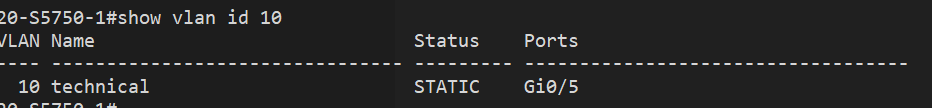
\includegraphics[width=13cm]{"./figure/2018-05-17-17-03-09.png"}
    \caption{查看vlan 10信息}
    \label{fig:e2-s2-see-vlan10}
    %\end{adjustwidth}
\end{figure}




\subsection{步骤3:交换机A创建VLAN20}

该步骤需要在交换机A上创建VLAN20,并将端口0/15(即PC2对应端口)划分到VLAN20中.

%\usepackage{changepage}
%\usepackage{rotating}
%\usepackage{float}
%\usepackage[section]{placeins}
%\begin{sidewaystable}[!Htp]
\begin{figure}[htp]
    %\begin{adjustwidth}{-1.5cm}{-1cm}
    \centering
    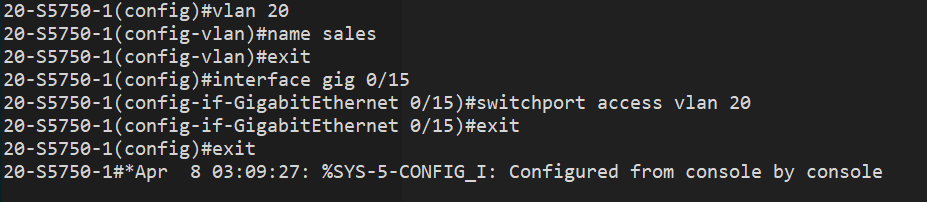
\includegraphics[width=13cm]{"./figure/2018-05-17-17-03-55.png"}
    \caption{创建VLAN20}
    \label{fig:e2-s3-vlan20}
    %\end{adjustwidth}
\end{figure}



操作完成后,使用\texttt{show vlan id 20}验证实验操作.

%\usepackage{changepage}
%\usepackage{rotating}
%\usepackage{float}
%\usepackage[section]{placeins}
%\begin{sidewaystable}[!Htp]
\begin{figure}[htp]
    %\begin{adjustwidth}{-1.5cm}{-1cm}
    \centering
    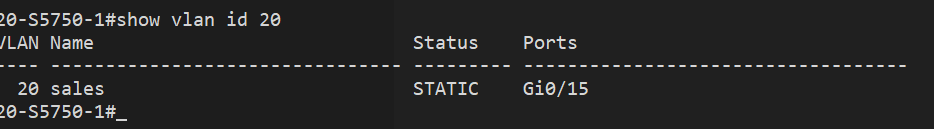
\includegraphics[width=13cm]{"./figure/2018-05-17-17-04-27.png"}
    \caption{查看VLAN20}
    \label{fig:e2-s3-see-vlan20}
    %\end{adjustwidth}
\end{figure}



\subsection{步骤4:设置A与B连接的端口模式}

将交换机A上与交换机B相连的端口(假设为端口0/24)定义为\texttt{tag VLAN}模式。设置步骤可见

%\usepackage{changepage}
%\usepackage{rotating}
%\usepackage{float}
%\usepackage[section]{placeins}
%\begin{sidewaystable}[!Htp]
\begin{figure}[htp]
    %\begin{adjustwidth}{-1.5cm}{-1cm}
    \centering
    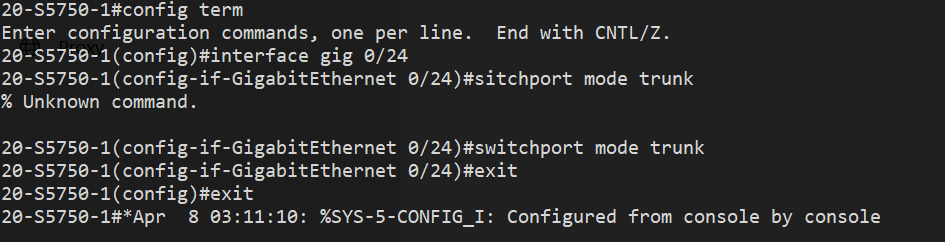
\includegraphics[width=13cm]{"./figure/2018-05-17-17-05-54.png
    "}
    \caption{设置端口模式}
    \label{fig:e2-s4-trunk}
    %\end{adjustwidth}
\end{figure}



操作完成后,使用\texttt{show interface gig 0/24 switchport}验证设置.
%\usepackage{changepage}
%\usepackage{rotating}
%\usepackage{float}
%\usepackage[section]{placeins}
%\begin{sidewaystable}[!Htp]
\begin{figure}[htp]
    %\begin{adjustwidth}{-1.5cm}{-1cm}
    \centering
    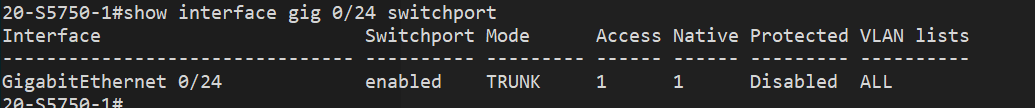
\includegraphics[width=13cm]{"./figure/2018-05-17-17-06-02.png"}
    \caption{验证设置}
    \label{fig:e2-s4-see-port}
    %\end{adjustwidth}
\end{figure}



\subsection{步骤5:交换机B创建VLAN20}

在交换机B上创建VLAN20,并将端口0/5划分到VLAN20中.如\autoref{fig:e2-s5-vlan20}

%\usepackage{changepage}
%\usepackage{rotating}
%\usepackage{float}
%\usepackage[section]{placeins}
%\begin{sidewaystable}[!Htp]
\begin{figure}[htp]
    %\begin{adjustwidth}{-1.5cm}{-1cm}
    \centering
    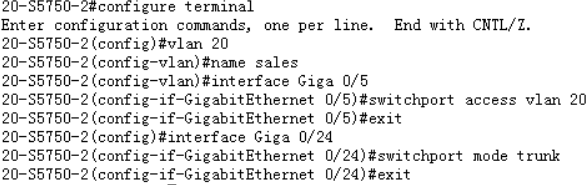
\includegraphics[width=13cm]{"./figure/2018-05-17-22-53-53.png"}
    \caption{交换机B创建VLAN20}
    \label{fig:e2-s5-vlan20}
    %\end{adjustwidth}
\end{figure}



操作完成后,使用\texttt{show vlan id 20}验证实验操作.如\autoref{fig:e2-s5-see-vlan20}

%\usepackage{changepage}
%\usepackage{rotating}
%\usepackage{float}
%\usepackage[section]{placeins}
%\begin{sidewaystable}[!Htp]
\begin{figure}[htp]
    %\begin{adjustwidth}{-1.5cm}{-1cm}
    \centering
    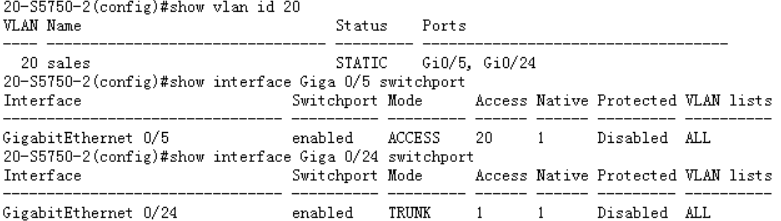
\includegraphics[width=13cm]{"./figure/2018-05-17-22-52-52.png"}
    \caption{在交换机B上查看vlan20}
    \label{fig:e2-s5-see-vlan20}
    %\end{adjustwidth}
\end{figure}


\subsection{步骤6:设置B与A连接的端口模式}


将交换机B上与交换机A相连的端口(假设为端口0/24)定义为\texttt{tag VLAN}模式。设置步骤可见\autoref{fig:e2-s6-port}


%\usepackage{changepage}
%\usepackage{rotating}
%\usepackage{float}
%\usepackage[section]{placeins}
%\begin{sidewaystable}[!Htp]
\begin{figure}[htp]
    %\begin{adjustwidth}{-1.5cm}{-1cm}
    \centering
    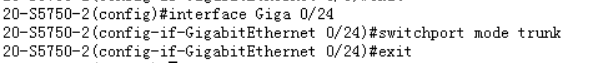
\includegraphics[width=13cm]{"./figure/2018-05-17-22-57-16.png"}
    \caption{设置端口模式}
    \label{fig:e2-s6-port}
    %\end{adjustwidth}
\end{figure}


操作完成后,使用\texttt{show interface gig 0/24 switchport}验证设置.见\autoref{fig:e2-s6-see-port}

%\usepackage{changepage}
%\usepackage{rotating}
%\usepackage{float}
%\usepackage[section]{placeins}
%\begin{sidewaystable}[!Htp]
\begin{figure}[htp]
    %\begin{adjustwidth}{-1.5cm}{-1cm}
    \centering
    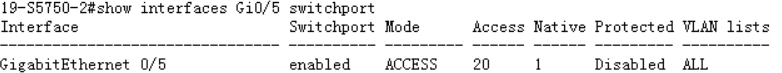
\includegraphics[width=13cm]{"./figure/2018-05-17-22-55-38.png"}
    \caption{设置端口模式}
    \label{fig:e2-s6-see-port}
    %\end{adjustwidth}
\end{figure}


\subsection{步骤7:测试}

\begin{enumerate}
    \item 测试PC2 与PC3 的连通性
    TODO:ping通截图 颜彬处

    \item 测试PC1 与 PC2 的连通性
    
    %\usepackage{changepage}
    %\usepackage{rotating}
    %\usepackage{float}
    %\usepackage[section]{placeins}
    %\begin{sidewaystable}[!Htp]
        \begin{figure}[htp]
            %\begin{adjustwidth}{-1.5cm}{-1cm}
            \centering
            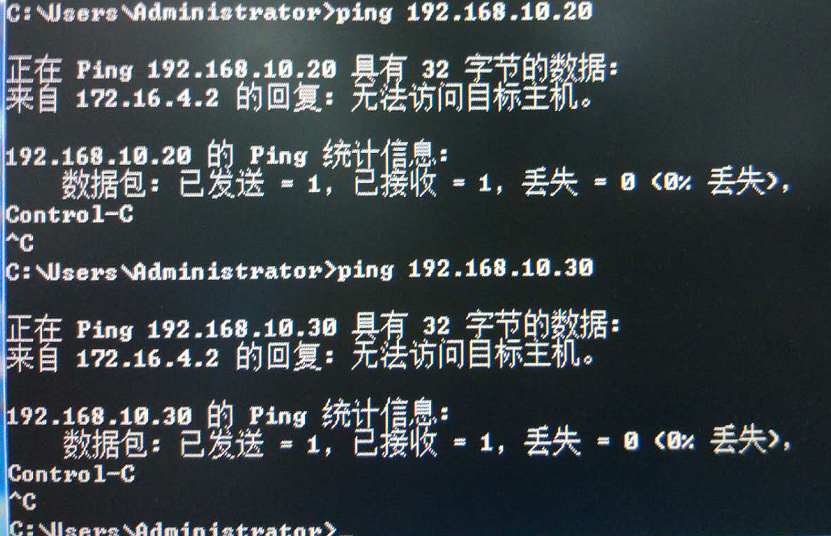
\includegraphics[width=13cm]{"./figure/2018-05-17-22-58-38.png"}
            \caption{PC1与PC2无法ping通}
            \label{fig:e2-s7-pc1-ping-pc3}
            %\end{adjustwidth}
        \end{figure}
        
    \item 使用\texttt{show ip route}命令查看三层交换机的路由表,并与步骤1比较.如\autoref{fig:e2-s7-route},步骤一中路由表可见\autoref{fig:e2-s1-route}。他们目前都是空的。
    %\usepackage{changepage}
    %\usepackage{rotating}
    %\usepackage{float}
    %\usepackage[section]{placeins}
    %\begin{sidewaystable}[!Htp]
    \begin{figure}[htp]
        %\begin{adjustwidth}{-1.5cm}{-1cm}
        \centering
        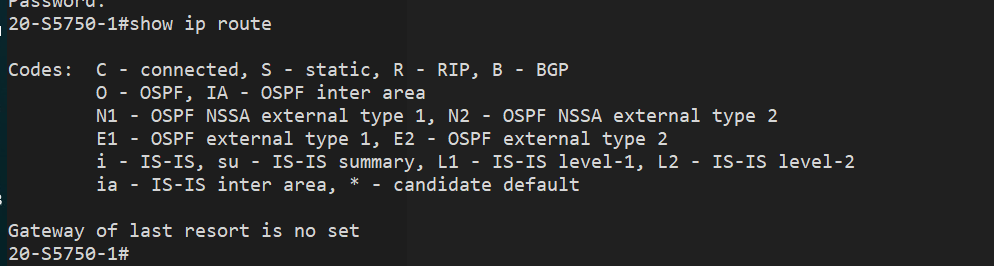
\includegraphics[width=13cm]{"./figure/2018-05-17-17-16-01.png"}
        \caption{查看路由表}
        \label{fig:e2-s7-route}
        %\end{adjustwidth}
    \end{figure}
    
    
\end{enumerate}


\subsection{步骤8:设置三层交换机VLAN间的通信}

将交换机A配置成具有路由器的功能,配置不同VLAN接口的地址.

%\usepackage{changepage}
%\usepackage{rotating}
%\usepackage{float}
%\usepackage[section]{placeins}
%\begin{sidewaystable}[!Htp]
\begin{figure}[htp]
    %\begin{adjustwidth}{-1.5cm}{-1cm}
    \centering
    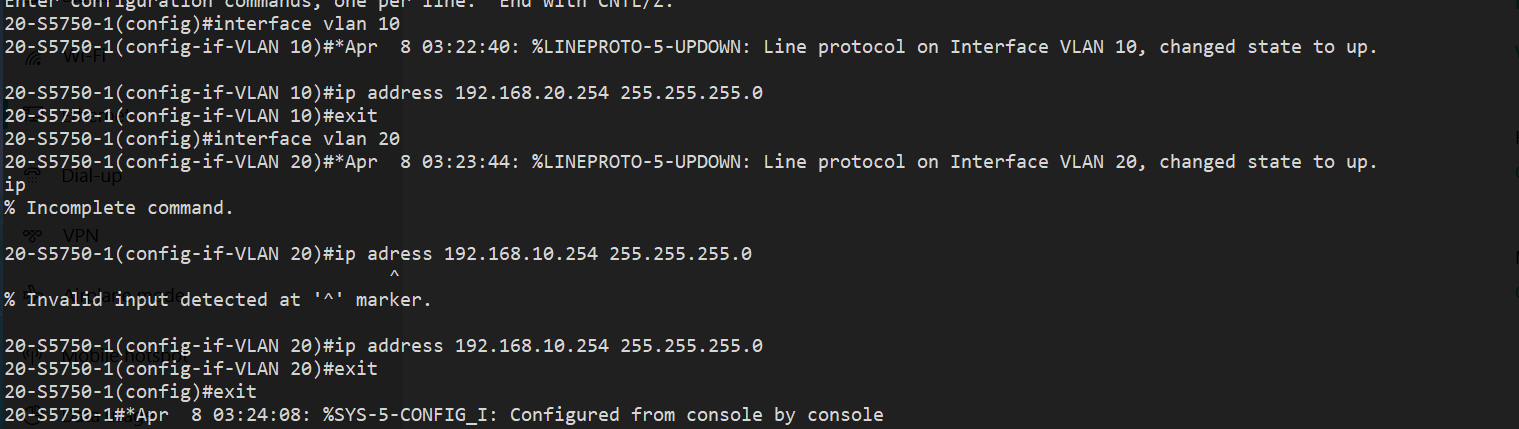
\includegraphics[width=13cm]{"./figure/2018-05-17-17-18-51.png"}
    \caption{设置vlan间通信}
    \label{fig:e2-s8-vlan}
    %\end{adjustwidth}
\end{figure}



%\usepackage{tcolorbox}
%\newtcolorbox{mybox}{}
%\renewtcolorbox{mybox}{colback = red!25!white, colframe = red!75!black}
%\begin{mybox}[title = {}]
\begin{tcolorbox}[title = {讨论}]
虚拟接口VLAN10与虚拟接口VLAN20的IP地址能不能在同一个网段?回答步骤1提出的问题.
\tcblower
不能.
如果在同一个子网中,主机不会尝试将这个数据包发往默认网关,这也就意味着交换机的路由模块无法收到这个数据包.
\end{tcolorbox}


\subsection{步骤9:设置网关}

该步骤设置网关可见步骤一,已经将VLAN 10和VLAN 20内的主机分别将默认网关设为\texttt{192.168.10.254}, \texttt{192.168.20.254}。

\subsection{步骤10:测试是否ping通}

实验测试,使用ping命令查看不同VLAN内的主机能够互相ping通.
启动监控软件Wireshark,互相ping两台计算机并观察.

关于此步骤结果,可见下一节"实验结果"。

\section{实验结果}

\subsection{实验观察}

%\usepackage{tcolorbox}
%\newtcolorbox{mybox}{}
%\renewtcolorbox{mybox}{colback = red!25!white, colframe = red!75!black}
%\begin{mybox}[title = {}]
\begin{tcolorbox}[title = {观察一}]
计算机之间是否连通?
\end{tcolorbox}

TODO:ping通的截图,三台都要
1. 我手机上PC1 pc2 PC3

%\usepackage{tcolorbox}
%\newtcolorbox{mybox}{}
%\renewtcolorbox{mybox}{colback = red!25!white, colframe = red!75!black}
%\begin{mybox}[title = {}]
\begin{tcolorbox}[title = {观察二}]
能否监控到PC1, PC2, PC3 的ICMP包?
\end{tcolorbox}

TODO:wireshark截图,并适当分析
颜彬的图

%\usepackage{tcolorbox}
%\newtcolorbox{mybox}{}
%\renewtcolorbox{mybox}{colback = red!25!white, colframe = red!75!black}
%\begin{mybox}[title = {}]
\begin{tcolorbox}[title = {观察三}]
使用\texttt{show ip route}查看三层交换机的路由表,并与步骤1比较.
\end{tcolorbox}

%\usepackage{changepage}
%\usepackage{rotating}
%\usepackage{float}
%\usepackage[section]{placeins}
%\begin{sidewaystable}[!Htp]
\begin{figure}[htp]
    %\begin{adjustwidth}{-1.5cm}{-1cm}
    \centering
    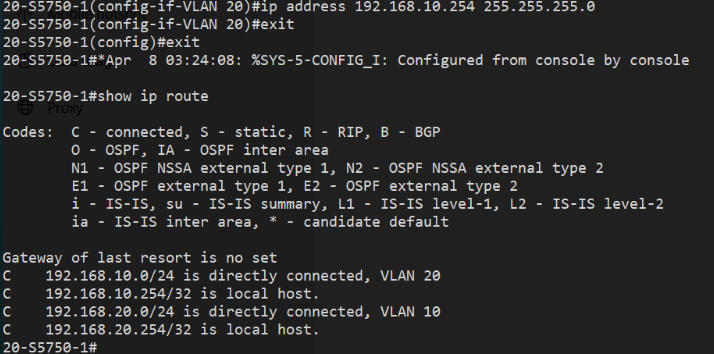
\includegraphics[width=13cm]{"./figure/2018-05-17-23-09-34.png"}
    \caption{三层交换机路由表}
    \label{fig:e2-s10-route}
    %\end{adjustwidth}
\end{figure}

与拓扑图比较,该路由表中的表项的意思为:TODO:wyf来写



%\usepackage{tcolorbox}
%\newtcolorbox{mybox}{}
%\renewtcolorbox{mybox}{colback = red!25!white, colframe = red!75!black}
%\begin{mybox}[title = {}]
\begin{tcolorbox}[title = {观察四}]
在命令提示符窗口下,使用route print 是否能够查看实验设置的路由?
\end{tcolorbox}

TODO:截图,分析wyf


\subsection{实验结论}
由本实验能得到什么结论?

TODO:??wyf
\begin{enumerate}
    \item 
    \item 
    \item 
    \item 
    \item 
\end{enumerate}

\section{实验思考}

思考题来自书本与老师提供的PDF材料.

\subsection{思考题一}

\begin{tcolorbox}[title = {思考题一}]
实验用到了三层交换机的路由功能,为什么在VLAN配置好IP地址之后,不同的VLAN间(PC1,PC2)就可以相互通信了?
\end{tcolorbox}

TODO:??wyf

\subsection{思考题二}

\begin{tcolorbox}[title = {思考题二}]
请使用\texttt{show ip route} 命令查看三层交换机的路由表,并说明每个条目表示什么?
\end{tcolorbox}

TODO:截图并分析wyf
figure/2018-05-17-17-26-19.png

\subsection{思考题三}

%\usepackage{tcolorbox}
%\newtcolorbox{mybox}{}
%\renewtcolorbox{mybox}{colback = red!25!white, colframe = red!75!black}
%\begin{mybox}[title = {}]
\begin{tcolorbox}[title = {思考题三}]
(跨交换机的不同vlan间通信)若要PC1和PC3相互通信,需要怎么进行配置.
\end{tcolorbox}

好像不用配置???

TODO:截图并分析

%%%%%%%%%%%%%%%%%%%%%%%%%%%%%%%%%%%%%%%%%%%%%%%%%%%%%%%%%%%%%%%%%%%%%%%%%%%%
% 参考文献
%%%%%%%%%%%%%%%%%%%%%%%%%%%%%%%%%%%%%%%%%%%%%%%%%%%%%%%%%%%%%%%%%%%%%%%%%%%%
% \cleardoublepage\phantomsection
% \addcontentsline{toc}{chapter}{参考文献}

% \bibliography{opsystem}
% \bibliographystyle{unsrt}

% \begin{thebibliography}{00}
%   \bibitem{r1} 作者. 文章题目 [J].  期刊名, 出版年份,卷号(期数): 起止页码.
%   \bibitem{r2} 作者. 书名 [M]. 版次. 出版地:出版单位,出版年份:起止页码.
%   \bibitem{r3} 邓建松等, 《\LaTeXe~科技排版指南》, 科学出版社.
%   \bibitem{r4} 吴凌云, 《CTeX~FAQ (常见问题集)》, \textit{Version~0.4}, June 21, 2004.
%   \bibitem{r5} Herbert Vo\ss, Mathmode, \url{http://www.tex.ac.uk/ctan/info/math/voss/mathmode/Mathmode.pdf}.
% \end{thebibliography}
%%%%%%%%%%%%%%%%%%%%%%%%%%%%%%%%%%%%%%%%%%%%%%%%%%%%%%%%%%%%%%%%%%%%%%%%%%%%
% 附录
%%%%%%%%%%%%%%%%%%%%%%%%%%%%%%%%%%%%%%%%%%%%%%%%%%%%%%%%%%%%%%%%%%%%%%%%%%%%
\appendix

\chapter{有附录吗?}

TODO:可能有附录,先留着?

\cleardoublepage
\end{document}